% TODO: ARRIVATO A PAGINA 20
% PARTITO DA PAG 28



\chapter{Intra-vehicle Communications}
% Bus systems: basics
%   Protocols
%   K-Line
%   CAN
%   LIN
%   FlexRay
%   MOST
%   In-car Ethernet
% ECUs
% Safety

\section{Bus Systems}

% \subsection{ISO/OSU Layers: Router}
%
% \begin{figure}[!ht]
%   \centering
%   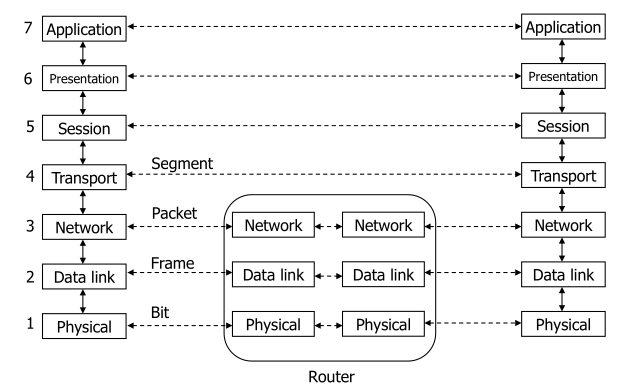
\includegraphics[width=0.4\textwidth]{./images/osi_router.png}
%   \caption{OSI Router}
%   \label{fig:osi_router}
% \end{figure}
%
% Da notare che se il router ha la parte di network separate, allora i due lati edllo strato network hanno protocolli diversi e il router deve fare da nterprete.
%
%
% \subsection{ISO/OSI Layers: Functions in Detail}
%
% \begin{itemize}
%   \item \textbf{Layer fisico}: trasmissione dei bit
%   \item \textbf{Layer data link}: trasmissione dei frame
%   \item \textbf{Layer network}: trasmette dei pacchetti
%   \item \textbf{Layer transport}: trasmissione sicura dei frammenti
%   \item \textbf{Layer session}: gestione della sessione
%   \item \textbf{Layer presentation}: definisce sintassi e semantica dell'informazione
%   \item \textbf{Layer application}: comunicazione fra applicazioni
% \end{itemize}



\subsection{Perchè usare i bus?}
Un bus che collega tutti i componenti al posto di avere una topologia a grafo completo ha i seguenti vantaggi:
\begin{itemize}
	\item \textbf{Riduzione dei costi}: meno cavi e meno connettori
	\item \textbf{Riduzione del peso}: meno cavi
	\item \textbf{Riduzione del volume}: meno cavi
	\item \textbf{Alta modularità}: modifica veicoli
	\item \textbf{Alta modularità}: cooperazione con OEM
	\item \textbf{Modularità}: riuso di moduli
	\item \textbf{Standardizzazione}: standardizzazione dei componenti e dei protocolli (meno errori scemi)
\end{itemize}




\subsection{Casi d'uso per intra-vehicle communications}

\begin{itemize}
	\item Driveline: Engine and transmission control
	\item Active Safety: Electronic Stability Programme (ESP)
	\item Passive Safety: Air bag, belt tensioners
	\item Comfort: Interior lighting, A/C automation
	\item Multimedia and Telematics: Navigation system, CD changer
\end{itemize}

La geolacaliuazione è fornita da protocolli di navigazione satellitare. I più famosi sono:
\begin{itemize}
	\item GPS: USA
	\item Galileo: EU
	\item Glonass: Russia
	\item Beidou: China
\end{itemize}

Altre soluzioni sono RTK(Real Time Kinematic)!!



\subsection{Classificazione: On-board-communcation}
\begin{itemize}
	\item Complex control and monitoring tasks: trasmissione dei dati tra ECUs(Engine Control Unit) e MMI(Man Machine Interface simile a HMI che sta per human machine interface)
	\item Simplification of wiring: rimpiazzare i fili di rame con bus per ridurre la complessità dei cablaggi
	\item Multimedia bus systems: Trasmette un sacco di dati per i sistemi di intrattenimento
\end{itemize}


\subsection{Classificazione: Off-board-communication(OBD connector)}
\begin{itemize}
	\item Diagnostics: diagnosi del veicolo
	\item Flashing: aggiornamento del software
	\item Debugging: debug del software
\end{itemize}

\subsection{Classificazione per casi d'uso e importanza}

\begin{table}[!ht]
	\begin{adjustbox}{width=\columnwidth,center}
		\begin{tabular}{|c|c|c|c|c|c|c|}
			\hline
			Application            & Message Length & Message rate & Data rate & Latency & Robustness & Cost \\
			\hline
			Control and monitoring &                & 2            & 2         & 3       & 3          & 2    \\
			\hline
			Simplified wiring      &                &              &           & 1       & 2          & 1    \\
			\hline
			Multimedia             & 1              & 2            & 3         & 1       & 1          & 3    \\
			\hline
			Diagnosis              &                &              &           &         &            & 1    \\
			\hline
			Flashing               & 2              &              & 2         &         & 1          &      \\
			\hline
			Debugging              &                & 1            & 1         & 2       &            &      \\
			\hline
		\end{tabular}
	\end{adjustbox}
	\caption{Classificazione per casi d'uso e importanza}
	\label{tab:classification_use_case}
\end{table}


\subsection{Classificazione SAE(Society of Automotive Engineers)}

\begin{table}
	\begin{adjustbox}{width=\columnwidth, center}
		\begin{tabular}{|c|c|c|c|}
			\hline
			Class & Data rate  & vantaggio                    & Dispositivi     \\
			\hline
			A     & $10kBit/s$ & Economico                    & Diagnosi        \\
			B     & $64kBit/s$ & Correzione errori            & Networking ECUs \\
			C     & $1MBit/s$  & Comunicazione in tempo reale & Drive train     \\
			D     & $10MBit/s$ & Bassa latenza                & X-By-Wire       \\
			\hline
		\end{tabular}
	\end{adjustbox}
	\caption{Classificazione SAE}
	\label{tab:classification_sae}
\end{table}



\subsection{Network Topologies}

\begin{itemize}
	\item \textbf{Repeter}: amplificazione del segnale a livello fisico
	\item \textbf{Bridge}: medium/timing adaptation, unfiltered forwarding a livello data link
	\item \textbf{Router}: medium/timing adaptation, filtered forwarding a livello network
	\item \textbf{Gateway}: medium/timing adaptation, filtered forwarding, protocol translation a livello application
\end{itemize}



\section{Bit coding}

Esistono due tipologie di encoding dell'informazione:
\begin{itemize}
  \item Non Return to Zero (NRZ)
  \item Manchester
\end{itemize}

Nella tipologia \textbf{NRZ} il valore logico $0$ è caratterizzato da un segnale basso, mentre il segnale logico $1$ è identificato da un segnale alto.

Nell'encoding di tipo \textbf{Manchester} si pone attenzione al cambio di livello per attribuire il valore logico, il valore logico $0$ è identificato dal passaggio da basso livello ad alto livello e il valore logico $1$ è identificato dal passaggio di stato da alto livello a basso livello.



\subsection{Reducing ElectroMagnetic Interference(EMI)}

\begin{itemize}
  \item Aggiungere schermatura ai fili
  \item usare fili twistati per coppie di fili(annullano effetti di elettromagnetismo a vicenda)
  \item Ridurre la ripidità del segnale
  \item usare usare NRZ che ha pochi cambi di stato
\end{itemize}

\subsection{Clock drift}

Il clock drift è causato dalla costruzione fisica del quarzo usato per il clock, che diffferensce leggermente da altri clock, questo fenomeno causa \textbf{desincronizzazione}.
\subsection{Bit stuffing}
Il problema associato all'utilizzo della codifica NRZ è che inviando una serie di bit costanti, in presenza di piccoli ritardi, i dati vengono ricevuti in maniera sbagliata.

Una soluzione proposta è quella del \textbf{Bit Stuffing} ed inserisce un bit extra dopo $n$ bit consecutivi.
\begin{itemize}
  \item Se ci sono 3 uni di fila, agiunge uno zero
  \item se ci sono 3 zeri di fila, aggiunge un uno
\end{itemize}


\section{Classification according to bus access}

\begin{figure}[!ht]
  \centering
  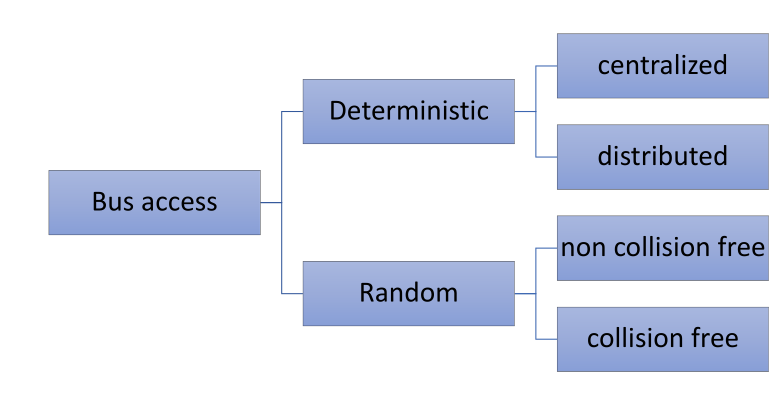
\includegraphics[width=0.4\textwidth]{./images/classification_bus_access.png}
  \caption{Classification according to bus access}
  \label{fig:classification_bus_access}
\end{figure}

\subsection{Deterministic}
\subsubsection{Centralized}
Accesso al bas di tipo \textbf{master-slave}(similare ad un sistema pooling)
\subsubsection{Decentralized}

Protocolli basati su \textbf{token}, tutti collegati a cerchio e si invia il messaggio con un token (che è tipo il bastone della parola) al ricevitore, il ricevitore manda il suo messaggio dopo nella catena insieme altoken e cosi via.

Solo il nodo con il token poò inviare il suo pacchetto di informazioni.


L'altro approccio è il \textbf{TDMA}(Time-division multiple access), si identificano i client attaccati al mezzo di comunicazione e si divide la comunicazioni a slot temporali e si può capire chi invia guardando il riferimento al clock

Grande problema di TDMA è la sincronizzazione.


\subsection{Random}
\subsubsection{Non Collision Free}
\textbf{CSMA/CA(Carrier Sense Multiple Access)/(Collision Avoidance)} misura l'energia del bus e invia quando l'energia è sotto un certo \textit{livello di riferimento}.

CSMA senza CA, se sente il canale occupato, seleziona un tempo random che chiama backoff e aspetta, dopo di che riprova ad ascolare il bus.

CSMA con CA ogni nodo conta il tempo che il noda che sta comunicando finisca, i nodi posso comunicare in qualsiasi momento e quindi ogni conteggio sarà diverso, dopo che il nodo ha finito di comunicare, ogni nodo aspetta il tempo che ha contato il precedenza.

se mentre i nodi stanno aspettando il tempo contato per trasmettere uno dei nodi finisce, si salva il tempo avanzato agli altri nodi e si utilizza quello per il prossimo check di chi tocca.

Questo sistema non è \textit{giusto} e può portare pacchetti a rimanere nella coda per tempi lunghi.



% TODO: descrivere meglio CSMA/CA

\textbf{CSMA/CD(Carrier Sense Multiple Access)/(Collision Detection)} se più nodi comunicano l'energia sul bus è maggiore del solito e i nodi si rendono conto del problema.

I nodi si fermano(per risparmiare risorse) e mandano un segnale \textbf{jamming} che è una sequenza di bit di alto livello per comunicare agli altri nodi il problema e di non comuniicare per un po.

Si applicano ai nodi dei tempi di backoff mediante strategie di backoff e si riprova.

\textbf{CSMA/CR(Carrier Sense Multiple Access)/(Collision Resolution)}:
\begin{enumerate}
  \item \textbf{Arbitration phase}: si compete per avere il canale
  \item \textbf{data}: il nodo che ha vinto il canale comunica
\end{enumerate}

E si itera questo processo ogni volta che un nodo vuole comunicare.


\subsection{Typical structure of an ECU}
\begin{figure}[!ht]
  \centering
  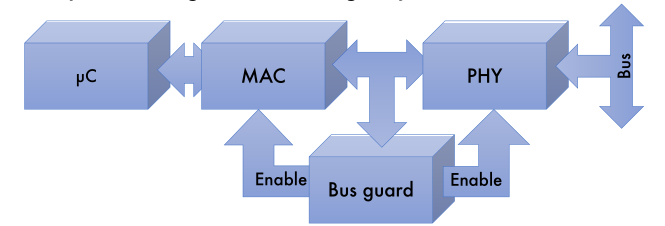
\includegraphics[width=0.4\textwidth]{./images/ecu.png}
  \caption{Struttura ECU}
  \label{fir:struttura_ecu}
\end{figure}





\section{Protocols}


\subsection{K-Like Bus}

Si concentra su \textbf{Layer fisico} e \textbf{Layer data link} ed è un bus bidirezionale con comunicazione su di un filo.


Principalmente usato per connettere:
\begin{itemize}
  \item ECU to Tester
  \item ECU to ECU
\end{itemize}

Lo \textbf{zero logico} ha un valore di energia inferiore al $20\%$ del massimo del bus, mentre il \textbf{uno logico} è rappresentato quando il segnale supera l'$80\%$ del valore massimo.

Questo protocollo è compatibile con \textbf{UART}(Universal Asynchronous Receiver Transmitter).




% TODO: GUARDARE DA PAGINA 46 A PAGINA 49 per scarsa attenzione


